\chapter{ Аналитический раздел}
\label{cha:analysis}

\textit{SDR(Standart Dynamic Range) изображение} -- изображение, пиксели которого содержат цвета и яркость, соответствующую глубине монитора.

\textit{LDR(Low Dynamic Range) изображение} -- изображение, пиксели которого хранят ограниченный диапазон цветов и яркости, предназначенное для отображении на старых мониторах.

\textit{HDR(High Dynamic Range) изображение} -- изображение, пиксели которого содержат более широкие значения цвета и яркости в сравнении с изображениями стандартного диапазона(SDR).

Получить HDR изображение можно получить несколькими способами: 
\begin{itemize}
    \item c помощью объединения снимков с разной длинной экспозиции,
    \item с помощью камеры, сенсор который позволяет захватить широкий объем данных,
    \item при помощи перевода LDR изображения в HDR специальными алгоритмами
\end{itemize}

Первый метод является более распространенным, так как устройства, которые больше всего распространены в повседневной жизни(телефоны, планшеты, веб-камеры) не обладают достаточно мощными сенсорами, для того, чтобы захватить широкий диапазон цветов. Последний метод не получил распространения, потому что задача перевода LDR или SDR изображения в HDR возможна только при помощи преминениями алгоритмов реконструкций, завязанных нейронных сетях, появивщихся достаточно недавно.

Задача получения HDR изображения не является тривиальной и делится на несколько этапов:
\begin{itemize}
    \item Выравнивание
    \item Реконструкция и удаление движущихся объектов
    \item Слияние кадров с разной экспозицией
    \item Преобразование HDR к LDR(tonemapping) если это требуется
\end{itemize}

\section{ Различия LDR и HDR изображений}

\textit{Глубина цвета} -- количество бит, приходящихся на один пиксель 
    
    Несмотря на то, что технологии за послдение несколько лет быстро развиваются и качество полученных кадров и устройств, их отображающих, увеличивается, получение картинки, сопоставимой с реальным окружением, остается нелегкой задачей. Яркость, диапазон цветов, которые видит человек в повседневной жизни, невозможно отобразить на большинстве мониторов, используещихся во всем мире. 

    Хотя уже начинают появлятся так называемые HDR мониторы и существуют камеры, сенсоры которых позволяют запечатлить широкий спектр цветов, яркостей и деталей, цена таких устройств может достигать огромных значений, поэтому большинство мониторов остаются SDR формата и не в состоянии передать картинку с большим количеством цветовой информации.

    Глубина цвета на большинстве мониторов составляет 8 бит. Глубина цвета самого распространенного формата изображений JPEG так же составляет 8 бит, в котором используется цветовое пространстов $YC_rC_b$. Это цветовое пространство позволяет использовать лишь малую часть видимых человеком цветов. Так же это цветовое пространство не способно передать большую часть яркостей, которых способен распознать человеческий глаз.

    В противовес формату JPEG существует так называемый RAW формат. В отличии от JPEG он способен содержать гораздо больше информации. Глубина цвета такого формата может достигать 12-16 бит(Значение может варьироваться в зависимости от возможностей сенсора камеры), который доступен в большинстве современных камер. Чаще всего этот формат автоматически переводят в JPEG во время съемки, что приводит к потере многих деталей без возможности восстановления. Однако, используя специальные инструменты RAW изображение в дальнейшем можно преобразовать в LDR изображение, получив на выходе кадр без потери нужной информации(провести tonemapping).

    На цветовом пространстве \ref{fig:hdrdiff} наглядно показан охват возможных отображаемых цветов в RGB пространстве или на тех же LDR мониторах и в HDR с глубиной цвета хотя бы в 12 бит.

\begin{figure}[ht!]
    \centering{
        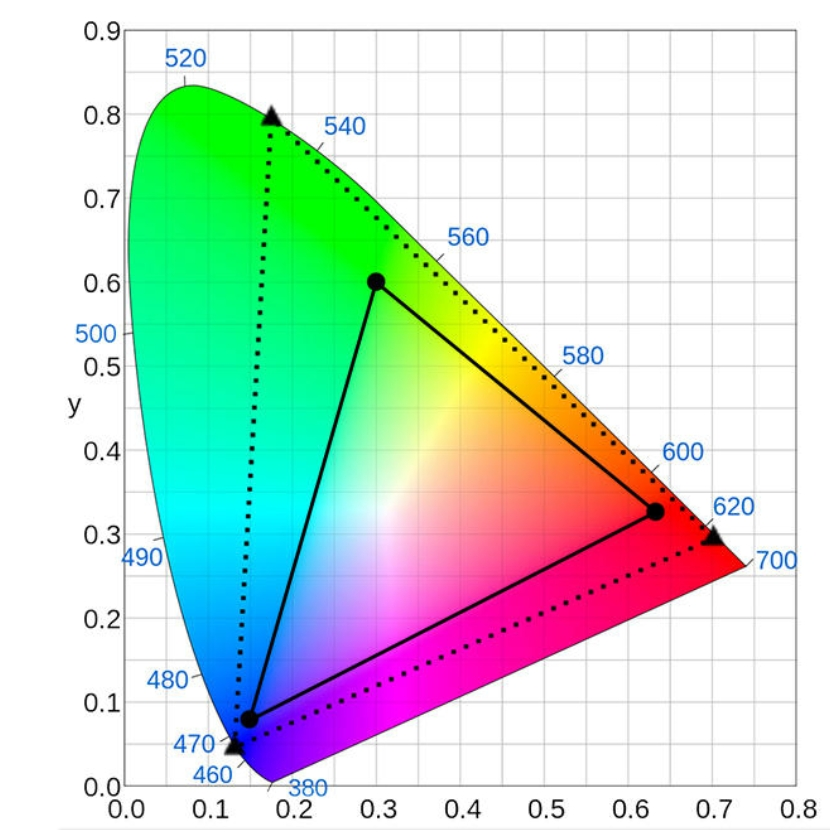
\includegraphics[width=0.4\textwidth]{img/rgb_vs_hdr_gamut.jpg}
	\caption{Охват видимых человеком цветов цветовым пространством RGB и HDR.}
        \label{fig:hdrdiff}
        }
\end{figure}

